\chapter{Conclusions}
\label{chap:discussion}
\newpage
\noindent
The aim of this thesis is the evaluation, development and application of robust methods to strengthen the raw material supply of a growing bio-economy sector. The success of bio-based companies depends, in part, on decisions that are made by foresters. Supporting forest management decisions is, therefore, beneficial, not only for the forest sector itself but also for wood processing companies. If forest enterprises and bio-economy companies are not able to contractually agree on continuous wood supply quantities, the success of a promising innovative bio-economy sector might be endangered. Forest decision-makers must, therefore, be very careful when deciding on the distribution of the available wood potential, as the downstream value creation process of the wood processing sector is much higher than the value creation in the forest sector itself \citep[p. 221, 223]{elchichakli_2016}. In a wood scarcity scenario, distribution decisions can have substantial consequences for wood processing companies, which depend on wood as a raw material. This reinforces the importance of DSS in the forest management decision process, as they can be used to structure the entire planning process of wood distribution into solvable sub-problems \citep[p. 1065-1067]{pretzsch_2008}. The benefits, disadvantages and results of the distinct statistical models developed here for decision support are discussed in the following.

\section{Findings of the thesis}
\label{sec:discussion:findings}
The introductory hypothesis, that matching demands of the rising bio-economy is actually problematic, was verified in chapter \ref{chap:hzb}. Scarcity of woody biomass and the high complexity of the entire wood supply chain are problems that forest enterprises and bio-economy companies have to cope with. A descriptive analysis of recent wood potential and wood usage reveals the significance of the research question and thus confirms the need for profound systems to help solve the anticipated raw wood distribution problem. After confirmation of the relevance of the introductory question in chapter \ref{chap:hzb}, the normative analysis in chapters \ref{chap:bm} to \ref{chap:opt} examine particular reasons why decision-makers may not be able to exploit the wood potential fully and how optimal potentials could be calculated.

\subsection{Analyzing status and development of raw wood availability in European beech-dominated central Germany}
\label{subsec:discussion:struct:hzb}
The available wood potential of all European beech wood assortments was almost completely exhausted in central Germany in the period between 2002 and 2012 (chapter \ref{chap:hzb}). Though the European beech wood potential is expected to rise due to ongoing forest development programs, competition on the wood market will probably rise. The only way for upcoming bio-economy companies to establish on the wood market is, thus, to compete with existing market participants. A detailed analysis of the wood market is, therefore, a prerequisite for the success of wood processing companies.

The added value of stem wood is higher than those of any other assortment \citep{nagel_2008}. The stem wood supply is currently entirely exhausted by long-established wood processing companies. It is therefore very difficult for novel companies to establish immediately on the stem wood market. Smaller-dimensioned, low-valued wood assortments make up about 60 \% of the available European Beech wood (chapter \ref{chap:hzb}). Although this low-valued wood is currently almost entirely used as well, availability is forecast to be better in the future. Approximately half of the wood potential of smaller dimension wood is directly used energetically. If a bio-economy company is able to compete with industrial wood and firewood prices, a solid base of renewable biomass from forests will then become available. This would be beneficial for the forest sector as well because the added value of sorting would increase \cite[p. 67]{mohring_1997}.

Two lessons should be learned from the predicted wood scarcity. First of all, the achievable sustainable wood potential should be estimated as accurately as possible in order to evaluate sources properly. Accurate estimations may uncover currently unused resources. Secondly, decisions on the distribution of the available wood potential must be made very carefully because the success of wood processing companies crucially depends on continuous wood supply quantities. Decisions on distribution of sparse resources can hence have serious consequences for forestry enterprises as well as for wood processing companies.

\subsection{Biomass functions and nutrient contents of European beech, oak, sycamore maple and ash and their meaning for the biomass supply chain}
\label{subsec:discussion:struct:bm}
The findings from chapter \ref{chap:bm} can improve harvest efficiency by making possible the gathering of the complete biomass potential of mixed broadleaf forest sites. A comparison of several existing models revealed that the introduced models can significantly improve the estimation accuracy of biomass and nutrient contents in mixed broadleaf tree species sites. This might help in identifying, and harvesting, formerly unused potential. The essay is particular relevant for the bio-based sector as innovative production methods often require biomass from broadleaf tree species \citep[p. 1]{auer_2016} and the frequency of mixed broadleaf stands is increasing steadily \citep{ti_2014}. The models enhance the accuracy of tree-specific biomass estimations. They can thus strengthen the planning accuracy of entire biomass supply chains.

\subsection{Modelling the economically viable wood in the crown of European beech trees}
\label{subsec:discussion:struct:beech_crowns}
The models from chapter \ref{chap:beech_crowns} are aimed at assessing the optimal wood volume in the crowns of European beech. They can thus be used to predict the full economically viable potential of smaller wood assortments. Allometric analysis revealed large wood potential in the crowns of broadleaf trees. It is therefore essential to consider the predicted wood volume from the crown, a by-product of stem wood production. As the dimension of the wood assortments plays a minor role for many activities (subsection \ref{subsec:intro:struct:bm}), gathering further wood potential from broadleaf crowns would seem to be of interest for bio-economy companies. The models also allow a precise prediction of harvestable wood volume prior to harvesting. They can therefore enhance the forecasting of volume flows in the biomass supply chain.

The model is able to calculate the maximal wood potential from an economic perspective only. It is therefore a purely normative-based model that predicts a rational, rather than a realistic, wood potential. Further economic or non-economic endogenous influences, such as fixed assortment lengths or maximum small-end diameters, cannot be considered in the model. It enables the calculation of the maximal tree-specific wood amount but it does not predict actual decisions.

\subsection{Flexible Global Optimization with Simulated-Annealing}
\label{subsec:discussion:struct:opt}
The optimization of forest stand treatments makes it possible to determine those forest operations with the highest marginal return (chapter \ref{chap:opt}). The model can be used to calculate the full wood potential of an entire forest enterprise in a time period of between 10 and 20 years. It is, in contrast to the other models mentioned, a model for the support of intermediate-term decisions on a lager spatial scale. The calculation of the full economic wood potential allows a sensitivity analysis of different optimization scenarios, which is of interest for planning purposes. If delivery agreements with upcoming bio-economy companies, or any other recipient, lead to opportunity costs, source providers must weigh the advantages and disadvantages very carefully. The optimization model enables the calculation of opportunity costs. The forest decision-maker can use the result to balance between the drawbacks of delivery contracts and their benefits in terms of planning security. They can decide whether the benefits in intermediate-term planning justify the opportunity costs. Furthermore, wood demanders can use the results to calculate adequate wood prices. The calculations can build an objective, evidence-based fundament for a binding agreement on intermediate-term wood prizes.

The combined si\-mu\-la\-tion-op\-ti\-mi\-za\-tion method makes high demands on the optimization algorithm (subsection \ref{subsec:intro:struct:opt}). A robust optimization procedure is a prerequisite for a reliable si\-mu\-la\-tion-op\-ti\-mi\-za\-tion model. Stochastic methods with dynamic random structures were able to cope with the specific needs of the combined si\-mu\-la\-tion-op\-ti\-mi\-za\-tion method. The best optimization is hence a composition of three optimization strategies \citep{corana_1987, kirkpatrick_1983, pronzato_1984}, which are all separately available as software packages. A composition of the two methods, simulation and optimization, is however, previously unpublished. The development of a specific software solution for the optimization of forest thinning activities was straightforward. An intensive sensitivity analysis confirmed the applicability and the efficiency of the package as the optimization element in the si\-mu\-la\-tion-op\-ti\-mi\-za\-tion software.

\subsection{Application of the forest harvesting schedule optimization}
\label{subsec:discussion:struct:opt:application}
\subsubsection{Introduction}
\label{subsubsec:discussion:struct:opt:application:introduction}
In this subsection, the two introduced practical examples (Subsection \ref{subsec:opt:examples:forest}) are described in detail. To explain its basic behavior and confirm its practical applicability, the si\-mu\-la\-tion-op\-ti\-mi\-za\-tion software was used to calculate optimized stand developments of two exemplary forest enterprises. These two examples explain how the model can be used to support the intermediate-term forest planning. The first exemplary enterprise was created to show the basic behavior of the simulation-optimization software. It is comprised of five systematically chosen forest stands. The stands of the second enterprise were chosen such that they represented a typical forest enterprise of central Germany. The second example explains the reasonability of the simulation-optimization approach for typical forest enterprises of the most important region for the supply European beech wood (Section \ref{sec:hzb:Einleitung}). It is hence reflects a common forest enterprise of the most important region for the wood supply of an upcoming wood-based bio-economy industry.

To explain the advantages of the simulation-optimization approach, the forest developments and the wood potentials of both enterprises were firstly foretasted without any optimization using the TreeGroSS packages. To perform a sensitivity analysis, a second scenario with optimized development using the simulation-optimization approach (Figure \ref{fig:Introduction:flowopt}) was calculated. In a third scenario, minimum harvesting volumes restrictions were implemented into the optimization system. The third scenario was performed to explain how the drawbacks of binding delivery contracts can be calculated via the si\-mu\-la\-tion-op\-ti\-mi\-za\-tion software.

\subsubsection{Materials and Methods}
\label{subsubsec:discussion:struct:opt:application:method}
Each exemplary forest enterprise was created using forest inventory data of a public forest district. The simulated stands were not 
The inventory data of intermediate-term forest planning built the data-base
 (see \ref{sec:intro:dss} for further details)
 
Unrestricted optimizations as well as optimization with delivery restrictions were performed on both enterprises using the introduced si\-mu\-la\-tion-op\-ti\-mi\-za\-tion approach (Section \ref{sec:intro:opt} and Chapter \ref{chap:opt}).

The first enterprise, which was used to explain the basic behavior of the optimization software, consisted of five European beech forest stands. The exemplary enterprise was used to demonstrate the practical applicability of the si\-mu\-la\-tion-op\-ti\-mi\-za\-tion software for typical forest enterprises.
Die 100 Bestande wurden zufallig gezogen. 100 mit Buche
\begin{table}[h]
	\centering
	\caption{Stand specific parameters of the first exemplary forest enterprise. The informations were generated with the stand summary function of the WaldPlaner \citep[p. 64]{hansen_2014}. dm: Diameter of stem of mean basal area. hm: Height of stem of mean basal area.}
	\label{my-label}
	\begin{tabular}{cccccccc}
		\hline
		stand              & species & 
		\begin{tabular}[c]{@{}c@{}}share\\ 	{[}\%{]} \end{tabular}
		
		& \begin{tabular}[c]{@{}c@{}} mean age\\ {[}a{]} \end{tabular} & 
		\begin{tabular}[c]{@{}c@{}} dm\\ {[}cm{]} \end{tabular} &
		\begin{tabular}[c]{@{}c@{}} hm\\ {[}m{]} \end{tabular} &  \begin{tabular}[c]{@{}c@{}}stand volume\\ {[}m$^3$ ha$^-1${]}\end{tabular} \\ \hline
		1                  & beech   & 100            & 52               & 14          & 21.3        & 215                                                                  \\
		2                  & beech   & 100            & 62               & 16          & 21.0        & 288                                                                  \\
		3                  & beech   & 100            & 102              & 30          & 28.3        & 381                                                                  \\
		4                  & beech   & 100            & 109              & 34          & 30.2       & 403                                                                  \\
		\multirow{2}{*}{5} & beech   & 66             & 69               & 18          & 22.9        & 113                                                                  \\
		& spruce  & 33             & 61               & 22          & 26.6       & 233                                                                  \\ \hline
	\end{tabular}
\end{table}
The second forest enterprise was composed of 100 forest stands with 560 ha of forest land. The stands of the second example were systematically chosen such that all economically relevant age classes of European beech are represented. The tree age distribution of the exemplary forest enterprise hence followed the characteristic distribution in European beech dominated central Germany (Figure \ref{fig:hzb:fig3_altersklassen}) covering all economically relevant age classes and tree species. The exemplary forest enterprise hence represented a typical enterprise of central Germany with usual species mixture and forest area (Chapter \ref{chap:hzb}; see also \citealp{ti_2014}).

\begin{table}[h]
	\centering
	\caption{Simulation settings of the standard treatment. The detailed listing of the specific tree species within the species groups can be found in \citet[p. 193-195]{hansen_2014}.}
	\label{tab:discussion:struct:opt:application:tab1}
	\begin{tabular}{cccc}
		\hline
		species group & \begin{tabular}[c]{@{}c@{}}target diameter\\ {[}cm{]}\end{tabular} & \begin{tabular}[c]{@{}c@{}}tree height at\\initial thinning\\ {[}m{]}\end{tabular} & \begin{tabular}[c]{@{}c@{}}number of future\\crop trees\\ {[}N ha$^{-1}${]}\end{tabular} \\ \hline
		oak         & 80 &14     & 80     \\
		European beech         & 60                                                                 & 16                                                                                  & 100                                                                                \\
		long-term deciduous trees           & 60                                                                 & 12                                                                                  & 80                                                                                 \\
		short-term deciduous trees           & 35-45                                                              & 10                                                                                  & 80                                                                                 \\
		spruce        & 45                                                                 & 12                                                                                  & 200                                                                                \\
		douglas fir     & 65                                                                 & 14                                                                                  & 120                                                                                \\
		pine        & 45                                                                 & 13                                                                                  & 180                                                                                \\
		larch        & 60                                                                 & 12                                                                                  & 120                                                                                \\ \hline
	\end{tabular}
\end{table}

The stands of the two exemplary forest enterprises 
All selected sites were located in the public forest district of Reinhausen \citep{nlf_2017}. Using the WaldPlaner import plug-in \citep[p. 58]{hansen_2014}, the official inventory data of Reinhausen were used to generate TreeGrOSS stands. The two exemplary forest enterprises thus both based on real forest stands from southern Lower Saxony. The stands were stored in a PostgreSQL data-warehouse \citep{eisentraut_2003}. The si\-mu\-la\-tion-op\-ti\-mi\-za\-tion software requires treatment settings that determine the standard scenario for the optimization. The respective options for the TreeGrOSS growth and yield simulation packages were developed by a work group of forest scientists and practitioners. The standard scenario represented the typical forest treatments in central Germany. Table \ref{tab:discussion:struct:opt:application:tab1} gives an overview of the crucial settings. With these stands and settings three scenarios were performed for each exemplary enterprise. Firstly, growth and yield of the exemplary enterprises were forecasted for 20 years using standard treatment configurations without optimization using TreeGrOSS (Figure \ref{fig:Introduction:flowopt}). After the simulation with these standard settings, the exemplary enterprises were forecasted with optimized treatments using the si\-mu\-la\-tion-op\-ti\-mi\-za\-tion software. The optimizations were  performed without minimum delivery restrictions to assess their entire wood potential for 20 years. In a third scenario, minimum delivery restrictions for low-dimensioned deciduous wood were defined to examine the impact of delivery contracts.

\textsc{\begin{figure}[h]
		\center
		\resizebox{1\linewidth}{!}{% Created by tikzDevice version 0.10.1 on 2017-05-28 17:18:03
% !TEX encoding = UTF-8 Unicode
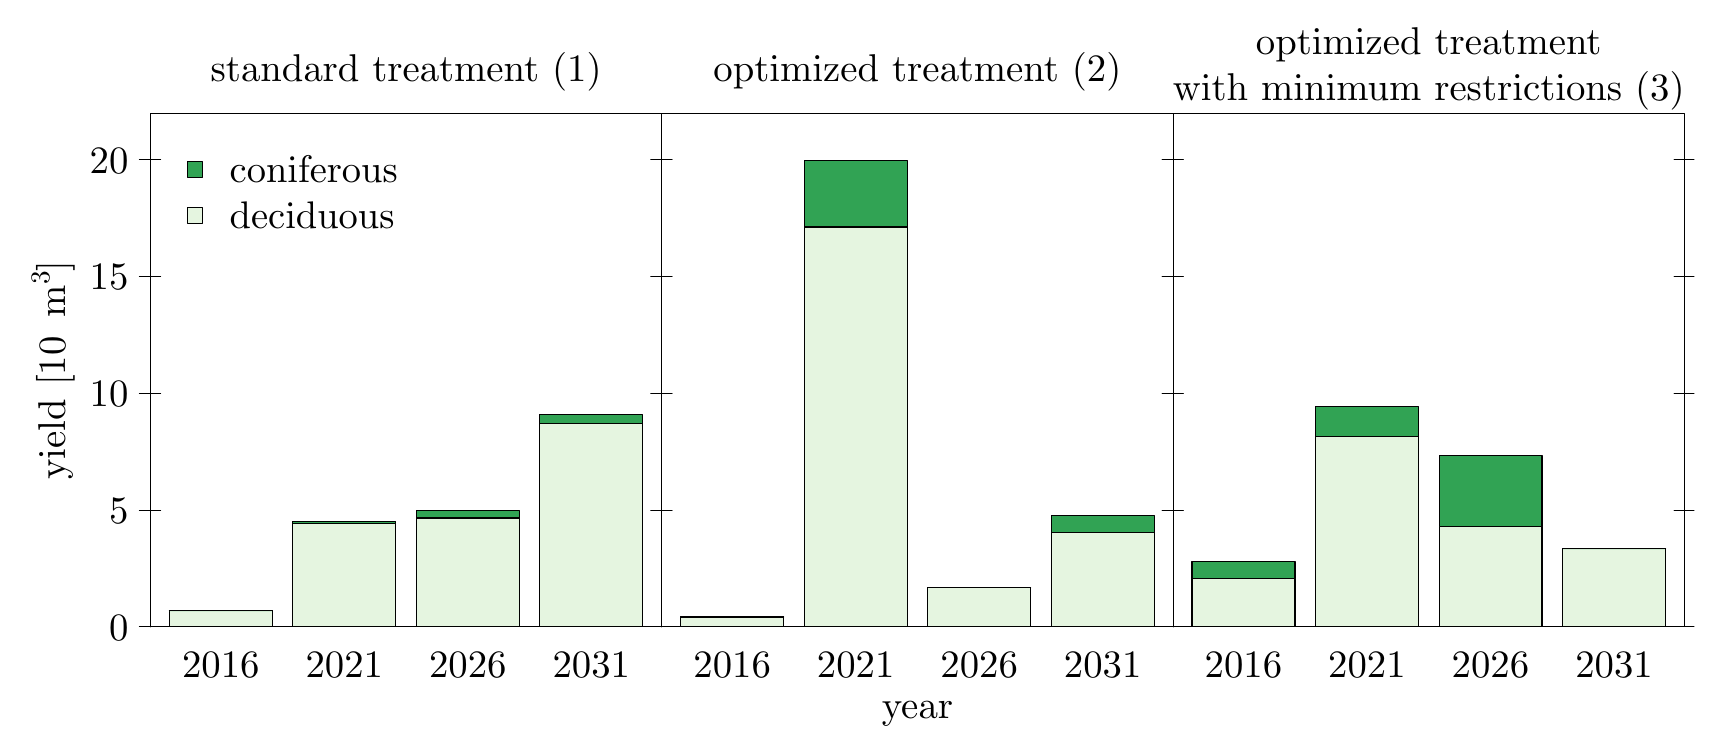
\begin{tikzpicture}[x=1pt,y=1pt]
\definecolor{fillColor}{RGB}{255,255,255}
\path[use as bounding box,fill=fillColor,fill opacity=0.00] (0,0) rectangle (602.23,252.94);
\begin{scope}
\path[clip] ( 44.35, 36.43) rectangle (229.12,222.06);
\definecolor{drawColor}{RGB}{0,0,0}
\definecolor{fillColor}{RGB}{229,245,224}

\path[draw=drawColor,line width= 0.4pt,line join=round,line cap=round,fill=fillColor] ( 51.20, 36.43) rectangle ( 88.39, 42.31);
\definecolor{fillColor}{RGB}{49,163,84}

\path[draw=drawColor,line width= 0.4pt,line join=round,line cap=round,fill=fillColor] ( 51.20, 42.31) rectangle ( 88.39, 42.31);
\definecolor{fillColor}{RGB}{229,245,224}

\path[draw=drawColor,line width= 0.4pt,line join=round,line cap=round,fill=fillColor] ( 95.83, 36.43) rectangle (133.02, 73.67);
\definecolor{fillColor}{RGB}{49,163,84}

\path[draw=drawColor,line width= 0.4pt,line join=round,line cap=round,fill=fillColor] ( 95.83, 73.67) rectangle (133.02, 74.64);
\definecolor{fillColor}{RGB}{229,245,224}

\path[draw=drawColor,line width= 0.4pt,line join=round,line cap=round,fill=fillColor] (140.46, 36.43) rectangle (177.65, 75.75);
\definecolor{fillColor}{RGB}{49,163,84}

\path[draw=drawColor,line width= 0.4pt,line join=round,line cap=round,fill=fillColor] (140.46, 75.75) rectangle (177.65, 78.43);
\definecolor{fillColor}{RGB}{229,245,224}

\path[draw=drawColor,line width= 0.4pt,line join=round,line cap=round,fill=fillColor] (185.09, 36.43) rectangle (222.28,109.94);
\definecolor{fillColor}{RGB}{49,163,84}

\path[draw=drawColor,line width= 0.4pt,line join=round,line cap=round,fill=fillColor] (185.09,109.94) rectangle (222.28,113.09);
\end{scope}
\begin{scope}
\path[clip] (  0.00,  0.00) rectangle (602.23,252.94);
\definecolor{drawColor}{RGB}{0,0,0}

\node[text=drawColor,anchor=base,inner sep=0pt, outer sep=0pt, scale=  1.40] at (136.74,233.66) {standard treatment (1)};

\path[draw=drawColor,line width= 0.4pt,line join=round,line cap=round] ( 44.35, 36.43) -- ( 40.39, 36.43);

\path[draw=drawColor,line width= 0.4pt,line join=round,line cap=round] ( 44.35, 78.62) -- ( 40.39, 78.62);

\path[draw=drawColor,line width= 0.4pt,line join=round,line cap=round] ( 44.35,120.81) -- ( 40.39,120.81);

\path[draw=drawColor,line width= 0.4pt,line join=round,line cap=round] ( 44.35,162.99) -- ( 40.39,162.99);

\path[draw=drawColor,line width= 0.4pt,line join=round,line cap=round] ( 44.35,205.18) -- ( 40.39,205.18);

\node[text=drawColor,anchor=base east,inner sep=0pt, outer sep=0pt, scale=  1.40] at ( 36.43, 31.61) {0};

\node[text=drawColor,anchor=base east,inner sep=0pt, outer sep=0pt, scale=  1.40] at ( 36.43, 73.80) {5};

\node[text=drawColor,anchor=base east,inner sep=0pt, outer sep=0pt, scale=  1.40] at ( 36.43,115.99) {10};

\node[text=drawColor,anchor=base east,inner sep=0pt, outer sep=0pt, scale=  1.40] at ( 36.43,158.17) {15};

\node[text=drawColor,anchor=base east,inner sep=0pt, outer sep=0pt, scale=  1.40] at ( 36.43,200.36) {20};

\path[draw=drawColor,line width= 0.4pt,line join=round,line cap=round] ( 44.35, 36.43) -- ( 48.05, 36.43);

\path[draw=drawColor,line width= 0.4pt,line join=round,line cap=round] ( 44.35, 78.62) -- ( 48.05, 78.62);

\path[draw=drawColor,line width= 0.4pt,line join=round,line cap=round] ( 44.35,120.81) -- ( 48.05,120.81);

\path[draw=drawColor,line width= 0.4pt,line join=round,line cap=round] ( 44.35,162.99) -- ( 48.05,162.99);

\path[draw=drawColor,line width= 0.4pt,line join=round,line cap=round] ( 44.35,205.18) -- ( 48.05,205.18);

\node[text=drawColor,anchor=base,inner sep=0pt, outer sep=0pt, scale=  1.40] at ( 69.79, 18.22) {2016};

\node[text=drawColor,anchor=base,inner sep=0pt, outer sep=0pt, scale=  1.40] at (114.42, 18.22) {2021};

\node[text=drawColor,anchor=base,inner sep=0pt, outer sep=0pt, scale=  1.40] at (159.05, 18.22) {2026};

\node[text=drawColor,anchor=base,inner sep=0pt, outer sep=0pt, scale=  1.40] at (203.68, 18.22) {2031};

\node[text=drawColor,rotate= 90.00,anchor=base west,inner sep=0pt, outer sep=0pt, scale=  1.40] at ( 13.53, 89.67) {yield [10};

\node[text=drawColor,rotate= 90.00,anchor=base west,inner sep=0pt, outer sep=0pt, scale=  1.40] at ( 13.53,141.37) { };

\node[text=drawColor,rotate= 90.00,anchor=base west,inner sep=0pt, outer sep=0pt, scale=  1.40] at ( 13.53,148.37) {m};

\node[text=drawColor,rotate= 90.00,anchor=base west,inner sep=0pt, outer sep=0pt, scale=  0.98] at (  7.80,160.04) {3};

\node[text=drawColor,rotate= 90.00,anchor=base west,inner sep=0pt, outer sep=0pt, scale=  1.40] at ( 13.53,164.94) {]};
\end{scope}
\begin{scope}
\path[clip] ( 44.35, 36.43) rectangle (229.12,222.06);
\definecolor{drawColor}{RGB}{0,0,0}
\definecolor{fillColor}{RGB}{49,163,84}

\path[draw=drawColor,line width= 0.4pt,line join=round,line cap=round,fill=fillColor] ( 57.76,198.95) rectangle ( 63.29,204.48);
\definecolor{fillColor}{RGB}{229,245,224}

\path[draw=drawColor,line width= 0.4pt,line join=round,line cap=round,fill=fillColor] ( 57.76,182.32) rectangle ( 63.29,187.84);

\node[text=drawColor,anchor=base west,inner sep=0pt, outer sep=0pt, scale=  1.39] at ( 73.00,196.94) {coniferous};

\node[text=drawColor,anchor=base west,inner sep=0pt, outer sep=0pt, scale=  1.39] at ( 73.00,180.31) {deciduous};
\end{scope}
\begin{scope}
\path[clip] (  0.00,  0.00) rectangle (602.23,252.94);
\definecolor{drawColor}{RGB}{0,0,0}

\path[draw=drawColor,line width= 0.4pt,line join=round,line cap=round] ( 44.35, 36.43) --
	(229.12, 36.43) --
	(229.12,222.06) --
	( 44.35,222.06) --
	( 44.35, 36.43);
\end{scope}
\begin{scope}
\path[clip] (229.12, 36.43) rectangle (413.89,222.06);
\definecolor{drawColor}{RGB}{0,0,0}
\definecolor{fillColor}{RGB}{229,245,224}

\path[draw=drawColor,line width= 0.4pt,line join=round,line cap=round,fill=fillColor] (235.97, 36.43) rectangle (273.16, 39.99);
\definecolor{fillColor}{RGB}{49,163,84}

\path[draw=drawColor,line width= 0.4pt,line join=round,line cap=round,fill=fillColor] (235.97, 39.99) rectangle (273.16, 39.99);
\definecolor{fillColor}{RGB}{229,245,224}

\path[draw=drawColor,line width= 0.4pt,line join=round,line cap=round,fill=fillColor] (280.60, 36.43) rectangle (317.79,180.91);
\definecolor{fillColor}{RGB}{49,163,84}

\path[draw=drawColor,line width= 0.4pt,line join=round,line cap=round,fill=fillColor] (280.60,180.91) rectangle (317.79,204.90);
\definecolor{fillColor}{RGB}{229,245,224}

\path[draw=drawColor,line width= 0.4pt,line join=round,line cap=round,fill=fillColor] (325.23, 36.43) rectangle (362.42, 50.69);
\definecolor{fillColor}{RGB}{49,163,84}

\path[draw=drawColor,line width= 0.4pt,line join=round,line cap=round,fill=fillColor] (325.23, 50.69) rectangle (362.42, 50.69);
\definecolor{fillColor}{RGB}{229,245,224}

\path[draw=drawColor,line width= 0.4pt,line join=round,line cap=round,fill=fillColor] (369.86, 36.43) rectangle (407.05, 70.62);
\definecolor{fillColor}{RGB}{49,163,84}

\path[draw=drawColor,line width= 0.4pt,line join=round,line cap=round,fill=fillColor] (369.86, 70.62) rectangle (407.05, 76.80);
\end{scope}
\begin{scope}
\path[clip] (  0.00,  0.00) rectangle (602.23,252.94);
\definecolor{drawColor}{RGB}{0,0,0}

\path[draw=drawColor,line width= 0.4pt,line join=round,line cap=round] (229.12, 36.43) -- (225.16, 36.43);

\path[draw=drawColor,line width= 0.4pt,line join=round,line cap=round] (229.12, 78.62) -- (225.16, 78.62);

\path[draw=drawColor,line width= 0.4pt,line join=round,line cap=round] (229.12,120.81) -- (225.16,120.81);

\path[draw=drawColor,line width= 0.4pt,line join=round,line cap=round] (229.12,162.99) -- (225.16,162.99);

\path[draw=drawColor,line width= 0.4pt,line join=round,line cap=round] (229.12,205.18) -- (225.16,205.18);

\path[draw=drawColor,line width= 0.4pt,line join=round,line cap=round] (229.12, 36.43) -- (232.82, 36.43);

\path[draw=drawColor,line width= 0.4pt,line join=round,line cap=round] (229.12, 78.62) -- (232.82, 78.62);

\path[draw=drawColor,line width= 0.4pt,line join=round,line cap=round] (229.12,120.81) -- (232.82,120.81);

\path[draw=drawColor,line width= 0.4pt,line join=round,line cap=round] (229.12,162.99) -- (232.82,162.99);

\path[draw=drawColor,line width= 0.4pt,line join=round,line cap=round] (229.12,205.18) -- (232.82,205.18);

\node[text=drawColor,anchor=base,inner sep=0pt, outer sep=0pt, scale=  1.40] at (254.56, 18.22) {2016};

\node[text=drawColor,anchor=base,inner sep=0pt, outer sep=0pt, scale=  1.40] at (299.19, 18.22) {2021};

\node[text=drawColor,anchor=base,inner sep=0pt, outer sep=0pt, scale=  1.40] at (343.82, 18.22) {2026};

\node[text=drawColor,anchor=base,inner sep=0pt, outer sep=0pt, scale=  1.40] at (388.45, 18.22) {2031};

\path[draw=drawColor,line width= 0.4pt,line join=round,line cap=round] (229.12, 36.43) --
	(413.89, 36.43) --
	(413.89,222.06) --
	(229.12,222.06) --
	(229.12, 36.43);

\node[text=drawColor,anchor=base,inner sep=0pt, outer sep=0pt, scale=  1.40] at (321.51,233.66) {optimized treatment (2)};

\node[text=drawColor,anchor=base,inner sep=0pt, outer sep=0pt, scale=  1.40] at (321.51,  3.17) {year};
\end{scope}
\begin{scope}
\path[clip] (413.89, 36.43) rectangle (598.66,222.06);
\definecolor{drawColor}{RGB}{0,0,0}
\definecolor{fillColor}{RGB}{229,245,224}

\path[draw=drawColor,line width= 0.4pt,line join=round,line cap=round,fill=fillColor] (420.74, 36.43) rectangle (457.93, 53.86);
\definecolor{fillColor}{RGB}{49,163,84}

\path[draw=drawColor,line width= 0.4pt,line join=round,line cap=round,fill=fillColor] (420.74, 53.86) rectangle (457.93, 59.96);
\definecolor{fillColor}{RGB}{229,245,224}

\path[draw=drawColor,line width= 0.4pt,line join=round,line cap=round,fill=fillColor] (465.37, 36.43) rectangle (502.56,105.28);
\definecolor{fillColor}{RGB}{49,163,84}

\path[draw=drawColor,line width= 0.4pt,line join=round,line cap=round,fill=fillColor] (465.37,105.28) rectangle (502.56,116.05);
\definecolor{fillColor}{RGB}{229,245,224}

\path[draw=drawColor,line width= 0.4pt,line join=round,line cap=round,fill=fillColor] (510.00, 36.43) rectangle (547.19, 72.60);
\definecolor{fillColor}{RGB}{49,163,84}

\path[draw=drawColor,line width= 0.4pt,line join=round,line cap=round,fill=fillColor] (510.00, 72.60) rectangle (547.19, 98.36);
\definecolor{fillColor}{RGB}{229,245,224}

\path[draw=drawColor,line width= 0.4pt,line join=round,line cap=round,fill=fillColor] (554.63, 36.43) rectangle (591.82, 64.58);
\definecolor{fillColor}{RGB}{49,163,84}

\path[draw=drawColor,line width= 0.4pt,line join=round,line cap=round,fill=fillColor] (554.63, 64.58) rectangle (591.82, 64.58);
\end{scope}
\begin{scope}
\path[clip] (  0.00,  0.00) rectangle (602.23,252.94);
\definecolor{drawColor}{RGB}{0,0,0}

\path[draw=drawColor,line width= 0.4pt,line join=round,line cap=round] (413.89, 36.43) -- (409.93, 36.43);

\path[draw=drawColor,line width= 0.4pt,line join=round,line cap=round] (413.89, 78.62) -- (409.93, 78.62);

\path[draw=drawColor,line width= 0.4pt,line join=round,line cap=round] (413.89,120.81) -- (409.93,120.81);

\path[draw=drawColor,line width= 0.4pt,line join=round,line cap=round] (413.89,162.99) -- (409.93,162.99);

\path[draw=drawColor,line width= 0.4pt,line join=round,line cap=round] (413.89,205.18) -- (409.93,205.18);

\path[draw=drawColor,line width= 0.4pt,line join=round,line cap=round] (413.89, 36.43) -- (417.59, 36.43);

\path[draw=drawColor,line width= 0.4pt,line join=round,line cap=round] (413.89, 78.62) -- (417.59, 78.62);

\path[draw=drawColor,line width= 0.4pt,line join=round,line cap=round] (413.89,120.81) -- (417.59,120.81);

\path[draw=drawColor,line width= 0.4pt,line join=round,line cap=round] (413.89,162.99) -- (417.59,162.99);

\path[draw=drawColor,line width= 0.4pt,line join=round,line cap=round] (413.89,205.18) -- (417.59,205.18);

\path[draw=drawColor,line width= 0.4pt,line join=round,line cap=round] (598.66, 36.43) -- (602.23, 36.43);

\path[draw=drawColor,line width= 0.4pt,line join=round,line cap=round] (598.66, 78.62) -- (602.23, 78.62);

\path[draw=drawColor,line width= 0.4pt,line join=round,line cap=round] (598.66,120.81) -- (602.23,120.81);

\path[draw=drawColor,line width= 0.4pt,line join=round,line cap=round] (598.66,162.99) -- (602.23,162.99);

\path[draw=drawColor,line width= 0.4pt,line join=round,line cap=round] (598.66,205.18) -- (602.23,205.18);

\path[draw=drawColor,line width= 0.4pt,line join=round,line cap=round] (598.66, 36.43) -- (594.97, 36.43);

\path[draw=drawColor,line width= 0.4pt,line join=round,line cap=round] (598.66, 78.62) -- (594.97, 78.62);

\path[draw=drawColor,line width= 0.4pt,line join=round,line cap=round] (598.66,120.81) -- (594.97,120.81);

\path[draw=drawColor,line width= 0.4pt,line join=round,line cap=round] (598.66,162.99) -- (594.97,162.99);

\path[draw=drawColor,line width= 0.4pt,line join=round,line cap=round] (598.66,205.18) -- (594.97,205.18);

\node[text=drawColor,anchor=base,inner sep=0pt, outer sep=0pt, scale=  1.40] at (439.33, 18.22) {2016};

\node[text=drawColor,anchor=base,inner sep=0pt, outer sep=0pt, scale=  1.40] at (483.96, 18.22) {2021};

\node[text=drawColor,anchor=base,inner sep=0pt, outer sep=0pt, scale=  1.40] at (528.59, 18.22) {2026};

\node[text=drawColor,anchor=base,inner sep=0pt, outer sep=0pt, scale=  1.40] at (573.22, 18.22) {2031};

\node[text=drawColor,anchor=base,inner sep=0pt, outer sep=0pt, scale=  1.40] at (506.28,243.30) {optimized treatment};

\node[text=drawColor,anchor=base,inner sep=0pt, outer sep=0pt, scale=  1.40] at (506.28,226.50) {with minimum restrictions (3)};

\path[draw=drawColor,line width= 0.4pt,line join=round,line cap=round] (413.89, 36.43) --
	(598.66, 36.43) --
	(598.66,222.06) --
	(413.89,222.06) --
	(413.89, 36.43);
\end{scope}
\end{tikzpicture}
}
		\caption{Simulated yield of the three different scenarios in 5-year periods, beginning with the period from 2011 to 2016. The yield is differentiated in coniferous and deciduous wood volume.}
		\label{fig:discussion:fig1}
	\end{figure}
}

\subsubsection{Discussion}
rh 5: 3. ist eine Umverteilung des Volumens von 1. 2. ist das beste aber entspricht nicht unbedingt den Waldbaurichtlinien

\section{Outlook}
\label{sec:discussion:outlook}
The next step will be to implement the developed and evaluated models into software for use by scientists, students and practitioners. The WaldPlaner DSS provides a favorable front-end for the models, as it is already established in forest science and used in practice.

One common aim of all the introduced methods is the assessment of the full wood potential from an economic perspective. All the models provide decision support to strengthen the economic forest function. There are, however, numerous good reasons not to fully exploit this potential. Conservation or recreational issues, which could decrease the actual harvestable wood volume, cannot be considered at present. Combinations of the models from chapters \ref{chap:bm} and \ref{chap:beech_crowns} with DSS could, however, enable consideration of other forest functions. Already existing forest DSS might reduce the wood potential due to conservation or recreational issues, thereby further enhancing the accuracy of predicted wood potentials. These aspects provide further arguments for an implementation of the introduced models into the WaldPlaner as the WaldPlaner allows parametrization of treatments with reduced wood potential \citep[p. 90-93]{hansen_2014}. Growth and yield simulations with nature conservation oriented treatment settings will forecast lower yields than economic oriented treatments. Combination of the presented methods from chapters \ref{chap:bm} and \ref{chap:beech_crowns} with the WaldPlaner hence enables forecasting of the stand specific wood potential with regard to economic and nature conservation issues.

The si\-mu\-la\-tion-op\-ti\-mi\-za\-tion software (chapter \ref{chap:opt}) optimizes the stand development with a view to economic issues. Consideration of the other two forest functions is nevertheless possible. As it was performed by \citet{yousefpour_2009}, conservation and recreational issues can be simplified such that they can be implemented as restrictions into the si\-mu\-la\-tion-op\-ti\-mi\-za\-tion software. Restrictions, such as harvesting permissions of old deciduous trees or minimum standing volumes for specific stand ages, could be included to enhance the forecasting accuracy in forest stands with specific nature conservation regulations. The influence of wood quality on the optimal stand treatment is another relevant issue that could be examined with the si\-mu\-la\-tion-op\-ti\-mi\-za\-tion software. To achieve this, an interface with user-specific wood prices must be implemented.

Cooperation between wood-processing companies themselves, as well as between the companies and forest enterprises, is the most important advantage for the bio-economy sector, where the assessment of complete raw material supply chains appears to be especially interesting. The methods introduced in this thesis were developed to help strengthen decisions in specific parts of supply chains, in order to promote the cooperation of the forest and the bio-economy sector. The statistical methods, however, cover only small, distinct parts of the supply chains. To enable meaningful cooperation, they must be somehow made applicable for decision-makers in forestry, as well as in bio-economy or logistic companies. When implementing the models into DSS, interfaces to other software will be mandatory in order to take full advantage of their potential. A front-end with an interface to logistic DSS could link the optimized wood amounts with resource distribution simulations or optimizations.